\documentclass{beamer}
\usepackage{xcolor}
\usepackage{fontspec}


% Standard colors
\definecolor{Red}{rgb}{1,0,0}
\definecolor{Blue}{rgb}{0,0,1}
\definecolor{Green}{rgb}{0,1,0}
\definecolor{Orange}{rgb}{1,0.65,0}
\definecolor{Black}{rgb}{0,0,0}

% Custom hex-based colors
\definecolor{DeepAquamarine}{HTML}{78DBE2}
\definecolor{DeepBlush}{HTML}{E36F8A}
\definecolor{DeepSaffron}{HTML}{FF9932}

% Set theme and colors
\setbeamercolor{background canvas}{bg=white}
\setbeamercolor{title}{fg=Blue}
\setbeamercolor{frametitle}{fg=Orange}
\setbeamercolor{normal text}{fg=Black}

% Fonts
\setmainfont{Times New Roman} % Default font for English
\newfontfamily\oriyafont{Odia Archana} % Font for Odia text

\begin{document}

% Slide 1: Title Slide
\begin{frame}
    \begin{center}
        \color{Orange}\Huge Cells, Genomes, and the Diversity of Life \\
        \vspace{0.5cm}
    \end{center}
\end{frame}

% Slide 2: Lack of Basic Infrastructure
\begin{frame}
    \frametitle{\color{Orange}\oriyafont ଜୀବ ଏକ ରାସାୟନିକ କାରଖାନା (organisms are chemical factories)}


- \color{Blue}{\oriyafont  ନିଜର ପ୍ରତିଲିପି (copies) ସୃଷ୍ଟି:} \color{Black} \oriyafont ଆମ ଗ୍ରହର ପୃଷ୍ଠ ଜୀବଜନ୍ତୁ - ଜୀବ - ଜଟିଳ ଭାବରେ ସଂଗଠିତ ରାସାୟନିକ କାରଖାନା ଦ୍ୱାରା ପରିପୂର୍ଣ୍ଣ, ଯେଉଁମାନେ ସେମାନଙ୍କ ପରିବେଶରୁ ପଦାର୍ଥ ଗ୍ରହଣ କରନ୍ତି ଏବଂ ଏହି କଞ୍ଚାମାଲ ବ୍ୟବହାର କରି ନିଜର ପ୍ରତିଲିପି (copies) ସୃଷ୍ଟି କରନ୍ତି।

- \color{Blue}{\oriyafont ଆମେ ବାହାରକୁ ଦେଖିଲେ ସମସ୍ତେ ଭିନ୍ନ। } \color{Black} \oriyafont ଜୀବମାନେ ଅସାଧାରଣ ଭାବରେ ବିବିଧ ଦେଖାଯାଆନ୍ତି। ପ୍ରଜାପତି, ଗଛ, ସାମୁଦ୍ରିକ ଘାସ, ବାଘ ସମସ୍ତେ ଭିନ୍ନ? ଆମେ ବାହାରଠାରୁ ଭିନ୍ନ ଦେଖାଯାଉ, ତଥାପି ଭିତରେ ଜୀବମାନଙ୍କର କାର୍ଯ୍ୟ ମୌଳିକ ଭାବରେ ସମାନ।

\end{frame}

\begin{figure}[h!]
    \centering
    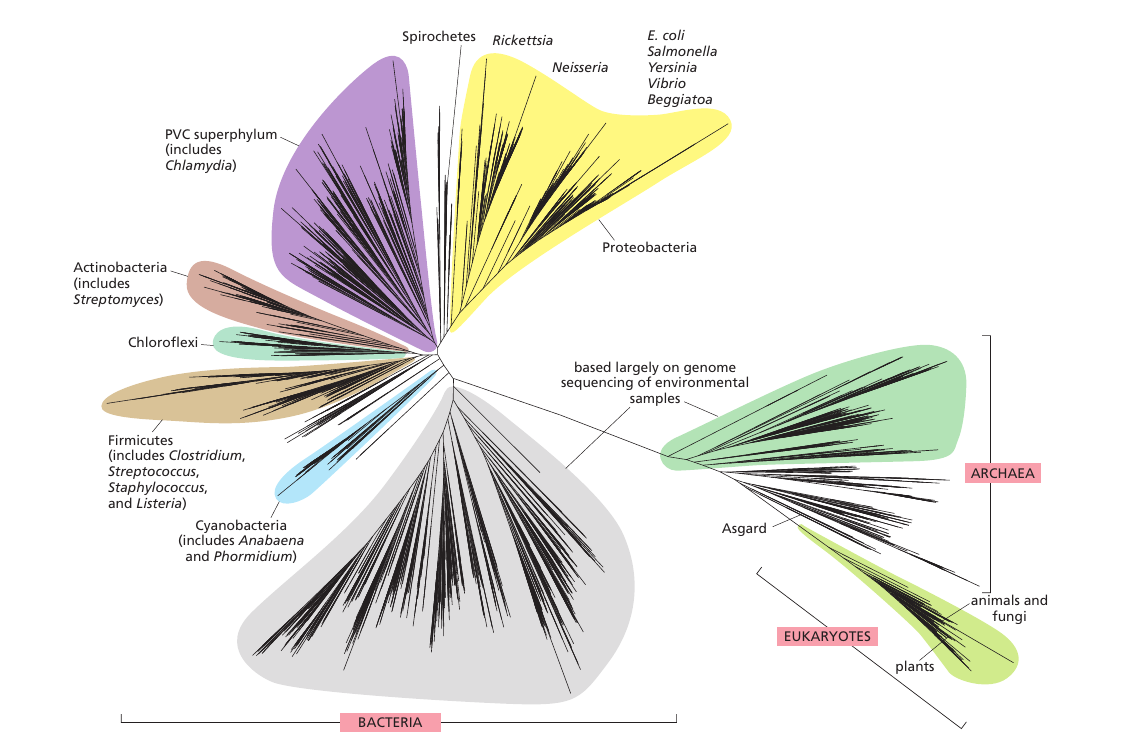
\includegraphics[width=0.9\textwidth]{domains.png} % Replace with your image file name
    \caption{\oriyafont ଜୀବ ଜଗତର ତିନୋଟି ପ୍ରମୁଖ ବିଭାଗ (ଡୋମେନ୍, domain)}
    \label{fig:sample-image}
\end{figure}

\end{document}
